\chapter{Opis stanowiska INTECO CRANE}
\label{inteco_stanowisko}

\section{Stanowisko TCRANE}
\label{inteco_stanowisko_TCRANE}
Trójwymiarowy model laboratoryjnego modelu dźwigu ilustruje strukturę współczesnego 
żurawia, skutecznie odwzorowuje stosunek wielkości do maksymalnego podnoszonego 
ładunku. Obiekt jest wielowejściowym i wielowyjściowym systemem wyposażonym w dedykowane
czujniki do mierzenia przemieszczeń i kątów.\\
\indent Stanowisko laboratoryjne T-Crane posiada 5 enkoderów inkrementalnych. Trzy z nich
mierzą położenie elementów napędzanych przez silniki. Dwa z nich znajdują się na karetce
dźwigu i przedstawiają aktualne wychylenie obciążenia od pionu.

\begin{figure}[H]
    \label{Opis::TCRANE::Stanowisko}
    \centering
    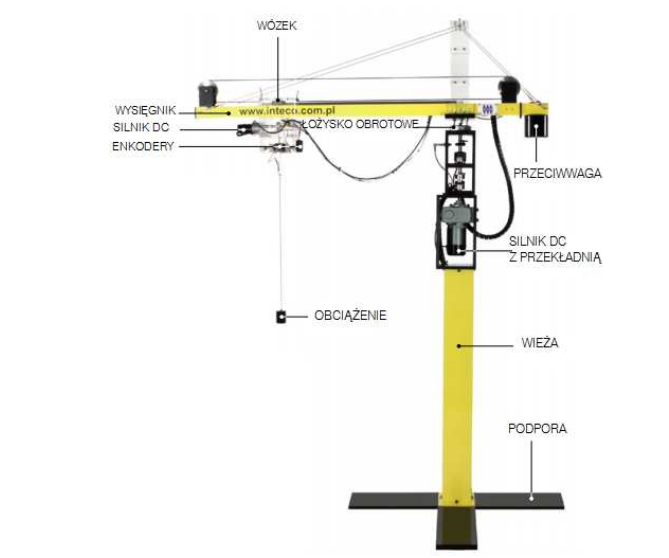
\includegraphics[scale=0.5]{./sections/inteco/images/tcrane.png}
    \caption{Stanowisko laboratoryjne TCRANE}
\end{figure}

W ramach projektu laboratoryjnego, mieliśmy wysterować ramię dźwigu w dwóch płaszczyznach:

\begin{itemize}
    \item obrót kolumny dźwigu (wieży)
    \item ruch wózka wzdłuż ramienia
\end{itemize}


\section{Wyznaczanie charakterystki statycznej}
\label{inteco_char_stat}
